\documentclass[conference]{IEEEtran}
\IEEEoverridecommandlockouts
% The preceding line is only needed to identify funding in the first footnote. If that is unneeded, please comment it out.
\usepackage{cite}
\usepackage{mathtools,amssymb,amsfonts,amsthm,bm}
\usepackage{algorithmic}
\usepackage{graphicx}
\usepackage{textcomp}
\usepackage{xcolor}
% Bibliography Package
	\usepackage[numbers]{natbib}
% Custom Packages
	\usepackage{tikz}
% Custom Commands
	\newcommand{\rx}{\mathsf{x}}
	\newcommand{\ry}{\mathsf{y}}
	\newcommand{\rs}{\mathsf{s}}
	\newcommand{\rz}{\mathsf{z}}
	\newcommand{\ru}{\mathsf{u}}
	\def\E{{\mathcal E}}
	\def\D{{\mathcal D}}
	\def\X{{\mathcal X}}
	\def\Y{{\mathcal Y}}
	\def\G{{\mathcal G}}
	\def\V{{\mathcal V}}
	\def\F{{\mathcal F}}
	\def\J{{\mathcal J}}
	\def\W{{\mathcal W}}
	\def\NN{{\mathbb N}}
	\def\QQ{{\mathbb Q}}
	\def\RR{{\mathbb R}}
	\def\ZZ{{\mathbb Z}}
	\def\FF{{\mathbb F}}
	\def\CC{{\mathbb C}}
	\def\mM{\bm{\mathrm{M}}}
	\def\mA{\bm{\mathrm{A}}}
	\def\mC{\bm{\mathrm{C}}}
	\def\mB{\bm{\mathrm{B}}}
	\newcommand{\QE}{\mathcal{Q}_{\mathrm{E}}}
	\newcommand{\QD}{\mathcal{Q}_{\mathrm{D}}}
	\newcommand{\oQE}{\overline{\mathcal{Q}}_{\mathrm{E}}}
	\newcommand{\oQD}{\overline{\mathcal{Q}}_{\mathrm{D}}}
	\newcommand{\BSS}{\mathrm{BSS}}
	\DeclareMathOperator{\Span}{Span}
	\newcommand{\rdummy}{{\color{red}[REF]}}
	\newcommand{\sdummy}{{\color{red}[SOURCE]}}
	\newcommand{\col}{\color{black}}
	\newcommand{\colol}{\color{orange}}
% Custom Environments
	\newtheorem{Theorem}{Theorem}
	\newtheorem{Definition}[Theorem]{Definition}
	\newtheorem{Lemma}[Theorem]{Lemma}
	\newtheorem{Corollary}[Theorem]{Corollary}
	\newtheorem{Remark}[Theorem]{Remark}
%	%	%	%	%	
\def\BibTeX{{\rm B\kern-.05em{\sc i\kern-.025em b}\kern-.08em
    T\kern-.1667em\lower.7ex\hbox{E}\kern-.125emX}}
\begin{document}
%
	\title{On the Decidability of the Remote State Estimation Problem on Blum-Shub-Smale Machines
	\thanks{{\color{red} Identify applicable funding agency here. If none, delete this.}}
	}

	\author{\IEEEauthorblockN{Holger Boche}
	\IEEEauthorblockA{\textit{Institute for}\\ 
	\textit{Theoretical Information Technology,}\\
	\textit{Technical University of Munich}\\
	Munich, Germany\\
	boche@tum.de\\
	\color{red} ORCID}
	\and
	\IEEEauthorblockN{Yannik Böck}
	\IEEEauthorblockA{\textit{Institute for}\\ 
	\textit{Theoretical Information Technology,}\\
	\textit{Technical University of Munich}\\
	Munich, Germany \\
	yannik.boeck@tum.de\\
	\color{red} ORCID}
	\and
	\IEEEauthorblockN{Christian Deppe}
	\IEEEauthorblockA{\textit{Institute for}\\
	\textit{Communications Engineering,}\\
	\textit{Technical University of Munich}\\
	Munich, Germany \\
	christian.deppe@tum.de\\
	\color{red} ORCID}
	}

\maketitle

\begin{abstract}
	We consider the descision problem associated to the remote state estimation of a dynamic plant. 
	That is, given the characteristics of some time-invariant, unstable, linear system, some linear sensor and some discrete, 
	memoryless channel (DMC), does there exist a pair of encoder and decoder that allows for the remote tracking of the system's 
	state with bounded error? Analytically, this problem has been shown to involve the eigenvalues of the plant's characteristics 
	and the zero-error capacity of the DMC. Starting from this result, we approach the problem from the view of theoretical computer science, 
	with an explicit treatment of the unerlying machine Model: does there exist a Blum-Shub-Smale computable algorithm that solves the above 
	decision problem based on the plant's and DMC's characteristics? Given the rise of digital technology in control and decision-making, 
	questions of this kind are becoming increasingly important, especially with regards to machine ethics and technology assessment. 
	Other than that, the problem has several unique features that make it noteworthy from a purely theoretical point of view. In light of the latter, we additionally
	investigate the problem for a slightly altered communication model, namely, an entanglement-assisted DMC. 
\end{abstract}

\begin{IEEEkeywords}
	\color{red} Keywords
\end{IEEEkeywords}

\section{Introduction}\label{sec:Introduction}
	\IEEEPARstart{R}{emote} state estimation is a prominent problem in control theory \sdummy.  

---

	-check usage of \(j,J,k,K,l,L,\ldots\).

---

	Informally, the corresponding dynamic system can be described as follows. The state of an unstable, linear, time-invariant plant is observed by a local sensor. 
	Subsequently, the sensor data is feed into an encoder that prepares the data for transmission trough a discrete, memoryless channel \emph{(DMC)}. 
	Based on the sequence of channel outputs, the remote decoder/estimator tries to estimate the current state of the plant. The setup is schematically depicted in Figure \ref{fig:Schematics} 
	(here, quantum-entanglement as a shared resource between encoder and decoder, which we will address in the further course of this section, is already included).
	\begin{figure}\linespread{1}
		\centering
		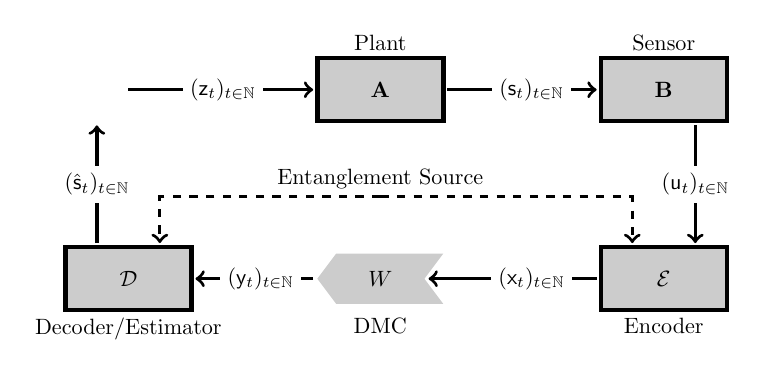
\begin{tikzpicture}[scale = 0.8, every node/.style={scale=0.8}]
			%   %   %   %   %   %   %   %   %   %   %
			%   Plant disturbance
				\draw[very thick, ->, shorten >=1.5pt] (-5,1.5) -- (-2,1.5); 
				\draw (-3.5,1.5)  node[fill = white, anchor=center, align=center]
				{\((\rz_t)_{t\in\NN}\)};
			%   %   %   %   %   %   %   %   %   %   %
			%   Plant
				\draw[ultra thick, fill=black!20] (-2,2) rectangle (0,1);
				\draw (-1,1.5)  node[anchor=center] {\(\mA\)};
				\draw (-1,2)  node[anchor=south] {Plant};
			%   %   %   %   %   %   %   %   %   %   %
			%   Plant -> Sensor
				\draw[very thick, ->, shorten >=1.5pt, shorten <=1.5pt] (0,1.5) -- (2.5,1.5); 
				\draw (1.4,1.5)  node[fill = white, anchor=center]
				{\((\rs_t)_{t\in\NN}\)};
			%   %   %   %   %   %   %   %   %   %   %
			%   Sensor
				\draw[ultra thick, fill=black!20] (4.5,2) rectangle (2.5,1);
				\draw (3.5,1.5)  node[anchor=center] {\(\mB\)};
				\draw (3.5,2)  node[anchor=south] {Sensor};
				
			%   %   %   %   %   %   %   %   %   %   %
			%   Sensor -> Encoder
				\draw[very thick, <-, shorten >=1.5pt, shorten <=1.5pt] (4,-1) -- (4,1); 
				\draw (4,0)  node[fill = white, anchor=center, align=center]
				{\((\ru_t)_{t\in\NN}\)};
			%   %   %   %   %   %   %   %   %   %   %
			%   Encoder
				\draw[ultra thick, fill=black!20] (4.5,-2) rectangle (2.5,-1);
				\draw (3.5,-1.5)  node[anchor=center] {\(\E\)};
				\draw (3.5,-2)  node[anchor=north] {Encoder};
			%   %   %   %   %   %   %   %   %   %   %
			%   Encoder -> Channel
				\draw[very thick, ->, shorten >=1.5pt, shorten <=1.5pt] (2.5,-1.5) -- (-0.3,-1.5); 
				\draw (1.4,-1.5)  node[fill = white, anchor=center, align=center]
				{\((\rx_t)_{t\in\NN}\)};
			%   %   %   %   %   %   %   %   %   %   %
			%   Channel
				\fill[fill = black!20] (-2,-1.5) -- (-1.7, -1.1) -- (0,-1.1) -- (-0.3,-1.5) -- (0,-1.9) -- (-1.7,-1.9);
				\draw (-1,-1.5)  node[anchor=center] {\(W\)};
				\draw (-1,-2)  node[anchor=north] {DMC};
			%   %   %   %   %   %   %   %   %   %   %
			%   Channel -> Decoder
				\draw[very thick, ->, shorten >=1.5pt, shorten <=1.5pt] (-2,-1.5) -- (-4,-1.5); 
				\draw (-2.9,-1.5)  node[fill = white, anchor=center, align=center]
				{\((\ry_t)_{t\in\NN}\)};
			%   %   %   %   %   %   %   %   %   %   %
			%   Decoder
				\draw[ultra thick, fill=black!20] (-6,-2) rectangle (-4,-1);
				\draw (-5,-1.5)  node[anchor=center] {\(\D\)};
				\draw (-5,-2)  node[anchor=north] {Decoder/Estimator};
			%   %   %   %   %   %   %   %   %   %   %
			%   State estimate
				\draw[very thick, ->, shorten >=1.5pt, shorten <=1.5pt] (-5.5,-1) -- (-5.5,1);
				\draw (-5.5,0)  node[fill = white, anchor=center, align=center]
				{\((\hat{\rs}_t)_{t\in\NN}\)};
			%   %   %   %   %   %   %   %   %   %   %    
			%   Entanglement Source
				\draw[very thick, dashed, ->, shorten >=1.5pt] (-1, -0.2) -- (-4.5, -0.2) -- (-4.5,-1);
				\draw[very thick, dashed, ->, shorten >=1.5pt] (-1, -0.2) -- (3, -0.2) -- (3,-1);
				\draw (-1,-0.2)  node[anchor=south] {Entanglement Source};
		\end{tikzpicture}
		\caption{Schematics of the remote state estimation setup considered throughout this article. Aside
					from the entanglement source, the setup is identical to the one introduced in \sdummy.}
		\label{fig:Schematics}
	\end{figure}
	
	In essence, the associated problem consists of designing a pair of encoder and decoder which allows for the estimation of the plant's state in a sufficient manner. 
	Prior to this, it is necessary to decide, based on the specifications of the plant and the DMC, whether an appropriate pair of encoder and decoder can exist in the first place. 
	Nowadays, this decision is often made by automated design tools or autonomous control units, e.g., in automated driving, either in an explicit or implicit way. In recent times, 
	\emph{digital twins} emerged as a further technique for handling design problems of this kind in practical applications. The approach is based on creating a full virtual copy of 
	the system on a digital computer, which is then employed for optimization, control tasks and decision-making. 

	From an analytic point of view, remote state estimation involves the disciplines of control and information theory. 
	The practice of automated design and autonomous control adds another layer to the problem. In almost all cases, dynamic plants are analog, continuous  systems, 
	whereas the operation of digital computers is based on discrete algorithms. Hence, the question of whether appropriate computer-based decision-making with respect to analog 
	dynamic systems is actually possible, arises naturally. 

	Problems of the latter kind are traditionally investigated in the field of theoretical computer science and have not gained much attention in applied engineering until now. 
	On the other hand, we can observe increasing requirements on electronic systems regarding safety, secrecy and, in lack of a different term, ethical behaviour \sdummy. 
	A prominent example is the related discussion surrounding autonomous driving, which is recently taking place in the community of machine ethics and technology assesment \sdummy. 
	In order to obtain a qualified evaluation of whether some digitally controlled technological system meets the abovementioned requirements, it is necessary to precisely understand 
	the fundametal boundaries of digital technology. This, in turn, requires an explicit treatment of those aspects of digital technology that involve theoretical computer science.

	In this series of articles (c.f. \sdummy for a full survey), we aim to approach the decision problem related to remote state estimation and stabilization from the perspective 
	of theoretical computer science. In \sdummy, we have considered the decision problem with regards to Turing machines. In this work, we instead discuss 
	\emph{Blum-Shub-Smale (BSS) machines} as the underlying machine model. Despite the {\color{red} fact \emph{(check styleguide!)}} that the capabilities real-world, digital computers are 
	entirely captured by Turing machines, BSS machines over \(\RR\) are {\color{red} regularly \emph{(check styleguide!)}} considered in numerics and computational complexity theory. 
	This practice is justified by the premise that the error emerging from representing real numbers by floating point approximations is neglectible in all practically relevant numerical problems. 
	Furthermore, assumptions on the underlying machine model are usually implicit in numerics. In contrast, we seek to explicitely treat the underlying machine model in our investigations.

	Regardless of any practical implications, the problem of remote state estimation has some features which make it unique from a theoretical point of view. As was shown in \sdummy, 
	the question of whether a suitable pair of encoder and decoder exists for a certain system specification involves the channel's zero-error capacity, a quantity itroduced in \sdummy. 
	To the best of the authors' knowledge, remote state estimation is the only egineering problem investigated so far which involves this quantity without explicitely requiring so in the 
	problem statement. The zero-error capacity itself has been subject to research for several years and gave rise to a number of mathematical problems. Several of these, for example, 
	the question of whether the zero-error capacity is always a Turing-computable number, are still unsolved. On the other hand, the zero-error capacity exhibits a list of noteworthy properties. 
	It has been shown that non-sginalling correlations, in particular, quantum-entanglement, can icrease the zero-error capacity. In turn, this suggests that there exist remote state estimation 
	configurations in which remote state estimation is possibe if the sender and the receiver share non-signalling correlations as a shared resource, but impossible if they don't. 

	The outline of the remainder of this work is as follows.

\section{Formal Description of the Remote State Estimation Setup}
	\noindent As indicated in Section \ref{sec:Introduction}, we consider the problem of remotely estimating the state of a dynamic plant via a noisy communication channel. 
	For a detailed treatment of the problem as such, we refer to \cite{MS07}. Schematically, the set-up is depicted in Figure \ref{fig:Schematics}. Aside from the entanglement source, 
	the system is identical to the one introduced in \sdummy. In order to provide a self-contained work, we recapitulate the description of the fully classical system given in \sdummy~ 
	alongside the entanglement-assisted case.

	The remote state estimation setup is characterized by the quintuple \((\mA,\mB,W,\E,\D)\) and the random variables \((\rz_t)_{t\in\NN}\), and \(\rs_{0}\). 
	The latter model the sequence of probabilistic fluctuations disturbing the plant, as well as the plant's initial state, respectively. The plant's state sequence \((\rs_t)_{t\in\NN}\) 
	and the sequence of sensor data \((\ru_t)_{t\in\NN}\) obey the system of equations
	\begin{align}	\rs_1    &= \mA \rs_0 + \rz_1, \\ 
					\rs_t    &= \mA \rs_{t-1} + \rz_t,\\ 
					\ru_t    &= \mB \rs_t,
	\end{align}
	where \(\mA\in\RR^{n\times n}\) and \(\mB\in\RR^{n\times l}\) capture the plant's and sensor's characteristics. 

	The sequence of channel inputs \((\rx_t)_{t\in\NN}\) is a sequence
	of symbols from a finite alphabet \(\X\). In the purely classical case, it is calculated by the encoder based on available sensor data,
	\begin{align}	\rx_t   &= \E \big(t, (\ru_{t'})_{t'=1}^{t}\big) \nonumber\\
							&= \E\big(t, \ru_1,\ru_2,\ldots,\ru_t\big).
	\end{align} 
	The sequence of channel outputs \((\ry_t)_{t\in\NN}\) is a sequence
	of symbols from a finite alphabet \(\Y\). In the classical case, it is component-wise related to the sequence \((\rx_t)_{t\in\NN}\) by a conditional probability mass function,
	\begin{align}   \label{eq:CndPrbMass}
					W :~ \Y \times \X \rightarrow [0,1],~(y,x) \mapsto W(y|x).
	\end{align}
	Last but not least, in the classical case, the decoder estimates the plant's state sequence based on the available channel outputs,
	\begin{align}	\hat{\rs}_t  	&= \D \big(t, (\ry_{t'})_{t'=1}^{t}\big) \nonumber\\ 
									&= \D\big(t,\ry_1,\ry_2,\ldots,\ry_t\big).
	\end{align}

	In the entanglement-assissted case, the encoding/decoding process is somewhat more involved. For \(n\in\NN\) arbitrary,
	we consider the Hilbert space
	\begin{align}	\mathfrak{H} := \bigotimes_{t = 1}^{\infty} \big(\mathbb{C}^{n}\otimes \mathbb{C}^{n}\big)
	\end{align}
	(for the construction of an infinite direct product, c.f. \sdummy), and for all \(t\in\NN\), the Hilbert spaces
	\begin{align}	\mathfrak{L}_{\mathrm{E}}^{(t)} :&= 
					\underset{\mathbb{C}}{\Span} \left\{\bigotimes_{t'=1}^{t}\hspace{2pt} \big(\mathrm{Id}(\CC^n) \otimes Q_{t'}\big) : Q_{t'} \in \mathbb{L}\big(\mathbb{C}^{n}\big)\right\}, \\
					\mathfrak{L}_{\mathrm{D}}^{(t)} :&= 
					\underset{\mathbb{C}}{\Span} \left\{\bigotimes_{t'=1}^{t}\hspace{2pt} \big(Q_{t'} \otimes \mathrm{Id}(\CC^n)\big) : Q_{t'} \in \mathbb{L}\big(\mathbb{C}^{n}\big)\right\}.
	\end{align}
	Futhermore, we denote by \(\mathfrak{L}_{\mathrm{E}+}^{(t)}\) and \(\mathfrak{L}_{\mathrm{D}+}^{(t)}\) the subsets of \(\mathfrak{L}_{\mathrm{E}}^{(t)}\) and 
	\(\mathfrak{L}_{\mathrm{D}}^{(t)}\), respectively, that consist of positive semi-definite operators on \(\mathfrak{L}_{\mathrm{E}}^{(t)}\) and \(\mathfrak{L}_{\mathrm{D}}^{(t)}\). 
	Then, the encoder and decoder are (positive) operator-valued mappings \(\QE\) and \(\QD\) that satisfy the following:
	\begin{itemize}	\item   For all numbers \(t \in \NN\), all sequences \((x_{t'})_{t'=1}^t\in\X^t\) and all sequences \((\ru_{t'})_{t'=1}^{t}\in (\RR^n)^t\), we have
						\begin{align}   \QE\Big((x_{t'})_{t'=1}^t\Big|t,(\ru_{t'})_{t'=1}^{t}\Big) \in \mathfrak{L}_{\mathrm{E}+}^{(t)}.
						\end{align}
					\item   For all numbers \(t\in \NN\), all sequences \((\hat{s}_{t'})_{t'=1}^{t}\in(\RR^n)^t\) and all sequences \((\ry_{t'})_{t'=1}^{t}\in\Y^t\), we have
						\begin{align}   \QD\Big((\hat{s}_{t'})_{t'=1}^{t}\Big|t,(\ry_{t'})_{t'=1}^{t}\Big) \in \mathfrak{L}_{\mathrm{D}+}^{(t)}.
						\end{align}
					\item   For all numbers \(t\in \NN\) and all sequences \((\ru_{t'})_{t'=1}^{t}\in (\RR^n)^t\), we have
						\begin{align}  \sum_{\bm{x}\in\X^t} \QE(\bm{x}|t,\ru_1,\ru_2,\ldots,\ru_t) = \mathrm{Id}\Big(\mathfrak{L}_{\mathrm{E}}^{(t)}\Big).
						\end{align}
					\item   For  all numbers \(t\in \NN\) and all sequences \((\ry_{t'})_{t'=1}^{t}\in \Y^t\), we have
						\begin{align}  \int_{(\RR^n)^t} \QD(\hat{s}|t,\ry_1,\ry_2,\ldots,\ry_t) \mathrm{d}\hat{\bm{s}} = \mathrm{Id}\Big(\mathfrak{L}_{\mathrm{D}}^{(t)}\Big).
						\end{align} 
	\end{itemize}
	We furthermore denote by \(\oQE\) and \(\oQD\) the identity-extension of \(\QE\) and \(\QD\), respectively, to \(\mathbb{L}(\mathbb{H})\), i.e.,
	\begin{align*}	&\oQE(x|t,\ru_1,\ru_2,\ldots,\ru_t) \\
					&\quad:=    \left(\bigotimes_{t'=t+1}^{\infty}\hspace{2pt} \mathrm{Id}(\CC^n\otimes\CC^n)\right) \otimes \QE(x|t,\ru_1,\ru_2,\ldots,\ru_t) \\
					&\oQD(\hat{s}|t,\ry_1,\ry_2,\ldots,\ry_t) \nonumber\\
					&\quad:=    \left(\bigotimes_{t'=t+1}^{\infty}\hspace{2pt} \mathrm{Id}(\CC^n\otimes\CC^n)\right) \otimes \QD(\hat{s}|t,\ry_1,\ry_2,\ldots,\ry_t)
	\end{align*}
	The encoding/decoding scheme also involves a rank-one projection operator on \(\mathbb{H}\), i.e, an operator \(\Psi\in\mathbb{L}(\mathbb{H})\) such that there 
	exists a vector \(\psi\in\mathbb{H}\) that satisfies 
	\begin{align}   \Psi(\bullet) = \psi \langle \psi, \bullet \rangle_{\mathbb{H}}.
	\end{align}

	The strong objective in remote state estimation requires almost sure observability. By a suitable choice of \(\E\) and \(\D\), the error between \((s(t))_{t\in\NN}\)
	and \((\hat{s}(t))_{t\in\NN}\) must be kept small along almost all possible trajectories \((\zeta(t))_{t\in\NN}\) and \((y(t))_{t\in\NN}\), i.e., with probability one. 
	Problems of this kind play an essential role in control theory \cite{BL00, EM01, HOV02, IF02, HT05, HF02, L03, MS04, MS05, MS05a, MS05b, PS01, S06, SP03, TM04, TM04b, WB99}. 
	However, it is commonly assumed that either the plant or the communication channel is noiseless, which neglects any uncertainty in the respective system components. 
	Hence, more realistic models for the remote state estimation problem incorporate noise-like disturbances in both the plant and the channel. 
	A corresponding framework was established in \cite{MS07}, which most of the considerations within the present work will be based on.
	In particular, the authors derived a strong relation between the solvability of the remote state estimation problem and the zero-error capacity \(C_0(W)\) of the 
	communication channel, as introduced in \cite{S56}. If the channel is unsuitable for transmitting a sufficient amount of data with perfect reliability, i.e., zero 
	chance of a transmission error, the discrepancy between \(s(t)\) and \(\hat{s}(t)\) accumulates over time and grows arbitrarily large, even if \((\zeta(t))_{t\in\NN}\) 
	is bounded arbitrarily close to zero. In this case, an unstable dynamic plant cannot be observed remotely with a bounded error. 

	In \cite{BD20Z}, the computability of \(C_0(W)\) in dependence of \(W\) is considered. Incorporating the results established in \cite{BD20Z}, 
	we want to investigate the remote state estimation problem with regards to algorithmic decidability. In particular...

\section{Introduction to the Theory of BSS Machines and Effective Analysis}
	{\color{red} Reference BSS Paper - }
	Blum-Shub-Smale (BSS) machines formalize the notion of computability over a field \(\FF\). The latter is assume to be equipped 
	with a binary relation \(\diamond~{:}~\FF \times \FF \rightarrow \{\mathsf{T},\mathsf{F}\}\), which is either an equality, equivalence or strict total order. 
	Despite the so called Church-Turing thesis being widely accepted as true, which implies that the capabilities of real-world computers are exactly characterized 
	by the abstract Turing machine, BSS machines are often implicitely considered as the underlying machine model in numerics and complexity theory \sdummy. 
	A reason for this practice may lie in the ability of BSS machines to handle exact real numbers. Since most areas of applied mathematics involve continuous structures, 
	treating the content of a computer's memory as actual real numbers simplifys the description of algorithms to a great extent. For a detailed discussion on the Topic, we refer to \sdummy.

	In essence, BSS machines can be considered a generalization of Turing machines. They are equipped with a two-way infinite tape divided into cells, each of which holds an 
	element of \(\FF\cup\{\sqcup\}\). Here, "\(\sqcup\)" denotes the distinguished empty-space symbol. We assume that the tape is almost empty, i.e., all but finitely many cells 
	contain the symbol "\(\sqcup\)", at the beginning of the computation. A BSS machine interacts with its tape by means of a read-write head, which can, depending on tis current 
	position, access a fixed number of contiguous cells at a time. The algorithm executed by the BSS machine is characterized by its programm, a finite, directed, simple graph 
	\begin{align}   \G_\BSS = ([M_\BSS]_{0}, \V_\BSS),~ \V_\BSS \subseteq [M_\BSS]_{0} \times [M_\BSS],
	\end{align} 
	with five types of nodes: \emph{input nodes}, \emph{computation nodes}, \emph{branching nodes}, \emph{shifting nodes} and \emph{output nodes}, each of which specifies a class 
	of fundamental machine operations. For a given input, the programm flow corresponds to a directed walk in the programm graph
	\begin{align}	\F := (e_t)_{t\in\{1,2,\ldots,T\}},~T\in\NN\cup \{\infty\},
	\end{align}
	starting from the input node and (possibly) ending in some output node, or continuing infinitely. In each step, the operaton associated to the current node is executed, 
	affecting the content of the tape, the position of the read-write head and the programm flow accordingly. Furthermore, the values stored in the initially non-empty cells 
	of the tape are considered part of the algoritm, much like hard-coded constants in a real-world computer programm. 

	In order to prove that some problem is BSS-computable, on has, in principle, to provide the existence of a suitable programm graph and, possibly, a tape with predefined constants. 
	This can often be cumbersome, since it involves the exact specification of the movement of the read-write head. If the size of the \emph{memory} required to execute the programm, i.e., 
	the number of different cells accessed througout the programm execution, can be uniformly upper bounded by a number \(J_\BSS \in \NN\), we can get rid of the tape alltogether by 
	introducing \emph{register variables} and \emph{constants},
	\begin{align}	\bm{r} :&= (r_j^t)_{j\in\{1,\ldots,J_{\mathrm{R}}\}, t\in\{1,\ldots,T\}},\\
					\bm{c} :&= (c_j)_{j\in\{J_{\mathrm{R}} + 1,\ldots,J_{\mathrm{C}}\}},
	\end{align}
	with \(T\in\NN\cup\{\infty\}\) and \(J_{\mathrm{C}} \leq J_\BSS\). The programm graph then consists only of an input node, computation nodes, branching nodes and at least one output node.
	Furthermore, the corresponding classes of fundamental machine operations can be specified as follows:
	\begin{itemize}	\item[1)] \emph{Input nodes.} The unique input node \(\iota = e_1 = 0\) is associated to an 
						input operation \(g_\iota\). The input operation writes each component of a tuple 
						\begin{align*} 	\bm{a} = \big(a_1,a_2,\ldots a_{K({\bm{a}})}\big) \in \bigcup_{j=1}^{J_{\mathrm{R}}} \FF^{j}
						\end{align*}
						to the machine's internal registers \(\bm{r}\), according to the specificaton
						\begin{align*}	r^1_{j(k)} := a_k ,~ j(k)\in \{1,\ldots,J_{\mathrm{R}}\},~ k\in \{1,\ldots K(\bm{x})\}.   
						\end{align*}
						The remaining registers are initialized with the value\linebreak \(0 \in \FF\).
						There exists a unique next node \(\iota' \in [M_\BSS]\) to \(\iota\).
					\item[2)] \emph{Computation nodes.} The programm graph may contain a number of computation nodes \(\zeta \in \{1,2,\ldots M_{\mathrm{C}}\}\),    
						\linebreak \(M_{\mathrm{C}} \leq M_{\BSS}\), each of which is 
						is associated to a mapping 
						\begin{align*} 	g_\zeta : \FF^{J_{\mathrm{C}}}\rightarrow \FF^{J_{\mathrm{R}}}. 
						\end{align*} 
						which is either polynomial, rational or has previously been shown to be BSS computable. The latter accounts for the fact that in the general, 
						unbounded setting, the programm of some BSS machine can always be incorporated as a subroutine into the programm of another BSS machine.
						If \(e_t = g_\zeta\) for some \(t\in\{1,\ldots, T-1\}\), we have
						\begin{align*}  \bm{r}^{t+1} = g_{\zeta}(\bm{r}^t,\bm{c})~\text{with}~\bm{r}^t := (r_j^t)_{j\in\{1,\ldots,J_{\mathrm{R}}\}}.
						\end{align*}
						There exists a unique next node \(\zeta' \in \{1,2,\ldots M_{\mathrm{C}}\}\) to each computation node \(\zeta\).
					\item[3)] \emph{Branching nodes.}  A programm may contain a number of branching nodes \(\beta \in \{M_{\mathrm{C}} + 1, M_{\mathrm{C}} + 2,\ldots, M_\mathrm{B}\}\), 
						each of which leave the content of the internal registers unchanged. That is, if \(e_t = \beta\) for some \(t\in\{1,\ldots, T-1\}\), we have
						\(\bm{r}^{t+1} = \bm{r}^{t}\). There exist exactly two next nodes \(\beta'(\mathsf{T})\) and \(\beta'(\mathsf{F})\) to each branching node \(\beta\). If 
						\begin{align*}	\diamond\big(0, r^t_{j'(\beta)}\big) = \mathsf{T} 
						\end{align*}
						holds true for \(j'(\beta) \in \{1,\ldots, J_\mathrm{R}\}\), the programm flow branches to the node \(\beta'(\mathsf{T})\). Otherwise, it moves to \(\beta'(\mathsf{F})\). 
						That is, for \(\beta = e_t\), we have
						\begin{align}   e_{t+1} =   \begin{cases}   \beta'(\mathsf{T})  &\text{if}~\diamond\big(0,r^t_{j'(\beta)}\big) = \mathsf{T},\\
																	\beta'(\mathsf{F})  &\text{otherwise}.
													\end{cases}    
						\end{align}
					\item[5)] \emph{Output nodes.} Each programm contains at least one output node \(\sigma \in \{M_{\mathrm{B}} + 1, M_{\mathrm{B}} + 2,\ldots, M_\BSS\}\), 
						each of which is associated to an output mapping
						\begin{align*}	o_\sigma : \FF^{J_{\mathrm{C}}}\rightarrow \FF^{J_{\sigma}}.
						\end{align*}
						For some fixed subset \(\J_\sigma\) of \([J_\mathrm{C}]\) and \(e_t = e_T = \sigma\), \(T\in\NN\), the mapping outputs (by projection) the values of the 
						register variables \((r_j^T)_{j\in \J_\sigma \cap \{1,\ldots,J_\mathrm{R}\}}\) and constants \((c_j)_{j\in \J_\sigma \cap \{J_\mathrm{R}+1,\ldots,J_\mathrm{C}\}}\). 
						There exists no next node to \(\sigma\).
	\end{itemize}
	In our case, the field \(\FF\) will be the real numbers \(\RR\) with the usual strict total order "\(<\)". If \(\FF\) equals \(\ZZ_2\) (the set of boolean values with logical con- and disjunction 
	as field operations), the traditional theory of computation as formalized by Turing machines is recovered. For the remainder of this article, we will refer to BSS machines over \(\RR\) 
	simply as BSS machines, omitting the explicit mention of the field \(\FF\) being equal to the real numbers. 

\section{Information Theory, Zero Error, Quantum Information Theory}
	For finite alphabets \(\X\) and \(\Y\), we consider conditional probability mass functions \(W\) that relate the elements of \(\X\) and \(\Y\) according to \eqref{eq:CndPrbMass}. 
	The triple \((\X,\Y,W)\) then characterizes a discrete, memoryless channel. 

	The theory of zero-error coding, as introduced in \sdummy, is a sub-discipline of general channel coding. Fundamentally, it considers the problem of finding the supremum 
	\(C_0(W)\) of all possible rates at which information can be transmitted trough a DMC \((\X,\Y,W)\) with perfect reliability. That is, given the channel output, the receiver must 
	be able to infer the transmitted data without any chance of error. In this context, the term "rate" refers to the asymptotic average of bits transmitted per channel use. 
	The number \(C_0(W)\) is commonly referred to as zero-error capacity of \(W\).

	In the following, for \(n\in\NN\) and \((\X,\Y,W)\) a DMC, denote by \(N(W,n)\) the maximum cardinality of a set \(\X'\subseteq \X^n\), such that for all \(\bm{x}^a,\bm{x}^b\in\X'\) 
	that satisfy \(\bm{x}^a \neq \bm{x}^b\), we have 
	\begin{align}	\sum_{\bm{y}\in\Y^n}\prod_{i=1}^{n} W(y_i|x_i^a)W(y_i|x_i^b) = 0.
	\end{align}

	\begin{Theorem} [\sdummy, {\color{red} remove the extra space!}]
					\label{Shannon}
					Let \((\X,\Y,W)\) be a discrete, memoryless channel. Then,
					\begin{align}	C_0(W)  &   = \limsup_{n\to\infty} \frac{1}{n} \log_2 N(W,n)\\
											&   = \lim_{n \to \infty} \frac{1}{n} \log_2 N(W,n),
					\end{align}
					is satisfied.
	\end{Theorem}

	The zero-error capacity of the DMC \((\X,\Y,W)\) can be characterized in terms of graph theory as well. For each channel \((\X,\Y,W)\), there exists a distinguished simple graph \(G(W)\), 
	which is referred to as confusability graph of the DMC \((\X,\Y,W)\). For details, see \sdummy. 

	\begin{Theorem}	[\sdummy]\label{thm:ZE_Capacity}
					For a DMC \(W\in\W(\X,\Y)\), let \(G(W) = (\X, \V(W))\) be the finite, simple graph that satisfies
					\begin{align}   \V(W) = \big\{\{x,x'\} : \exists y : W(y|x)W(y|x') > 0\big\}.
					\end{align}
					Then, the zero-error capacity of \(W\) satisfies
					\begin{align}   C_0(W)  &=  \lim_{n\to\infty} \frac{1}{n} \log_2 \alpha\big(G^{\boxtimes n }(W)\big) \\
											&=  \sup_{n\in\NN} \frac{1}{n} \log_2 \alpha\big(G^{\boxtimes n }(W)\big),
					\end{align}
					where \(G^{\boxtimes n }(W)\) denotes the \(n\)-fold \emph{strong graph product} of \(G(W)\) with itself and
					\(\alpha\big(G^{\boxtimes n }(W)\big)\) denotes the \emph{independence number} of \(\alpha\big(G^{\boxtimes n }(W)\big)\).
	\end{Theorem}


\section{BSS Computability of Zero-Error and EAZE Capacity}\label{State}
	In the following, we specify a BSS-Algorithm which, for fixed alphabets \(\X\) and \(\Y\), computes the zero-error capacity \(C_0(W)\) upon being passed a channel description \(W \in \W_c(\X,\Y)\). 

	Essentially, algorithm relies on the fact that a \emph{lookup table} containing all possible values of \(C_0(W)\) can be hard-coded into the programm. The lookup is performed in 
	terms of a perfect binary tree, where each branch corresponds to an evaluation of the predicate "\(W(y|x) > 0\)" for some letters \(x\in\X\) and \(y\in\Y\). Per definition, the latter 
	can be done algorithmically, as a fundamental operation on the BSS machine.

	\begin{Theorem}	Consider finite alphabets \(\X\) and \(\Y\). Then, there exists a BSS-Machine \(\BSS_{C_0}\)
					which, upon being passed a channel description \(W\in \W_c(\X,\Y)\), computes the mapping \(W \mapsto C_0(W)\).
	\end{Theorem}\begin{proof}
					Let \(j \mapsto \big(x(j), y(j)\big)\) be an enumeration of the set \(\X\times\Y\) and define
					\(J_\mathrm{R} := |\X\times \Y|\). Furthermore, consider the mappings
					\begin{align}	\delta(W,j) :&=     \begin{cases}   1   &\text{if}~ 0 < W\big(y(j)|x(j)\big), \\
																		0   &\text{otherwise},
														\end{cases}\\
									\Delta(W)   :&=     1 + \sum_{j=1}^{J_\mathrm{R}} \delta(W,j)\cdot 2^{j-1} \in \big\{1,\ldots,2^{J_\mathrm{R}}\big\}.
					\end{align} 
					We observe that, as a direct consequence of Theorem \ref{thm:ZE_Capacity}, the value of \(C_0(W)\) is 
					entirely determined by the set 
					\begin{align}   \{(x,y) \in \X\times \Y : W(x|y) > 0\} \subseteq 2^{\X\times\Y}
					\end{align} 
					and hence, the zero-error capacity of \(W\) depends exclusively on the number \(\Delta(W)\). Thus, we obtain the existence of a mapping
					\begin{align}	C'_0 : \big\{1,\ldots,2^{J_\mathrm{R}}\big\} \rightarrow \RR_0^+,~ \Delta \mapsto C'_0(\Delta)        
					\end{align}
					such that \(C'_0(\Delta(W)) = C_0(W)\) holds true for all \(W\in\W(\X,\Y)\). For \(J_\mathrm{C} := J_\mathrm{R} + 2^{J_\mathrm{R}}\), 
					hardcode the family of constants \(\bm{c}\) according to 
					\begin{align}   c_j := C'_0(j - J_\mathrm{R})
					\end{align}
					for all \(j\in \{J_\mathrm{R} + 1, \ldots, J_\mathrm{C}\}\) and specify the programm \(\G = ([M_\BSS],\V_\BSS)\) with
					\begin{align}	M_\mathrm{C} := 0,~M_\mathrm{B} := 2^{J_\mathrm{R}} - 1,~ M_\BSS := ~M_\mathrm{B} + 2^{J_\mathrm{R}}
					\end{align}
					in the following way:
					\begin{enumerate}	\item[\(\iota\)\hspace{1pt}:] Preallocate the machine's registers \(\bm{r} := \bm{r}^1\) according to
											\(r_j := r^1_j := W\big(y(j)|x(j)\big)\). Since the programm does not contain any computation nodes,
											the content of the registers remains constant during the execution. We thus omit the superscript of the
											register variables in the following.
										\item[\(\beta\)\hspace{1pt}:] 
											For \(\beta \in \{1,\ldots, M_\mathrm{B}\}\), the pair of next nodes \(\big(\beta'(\mathsf{T}),\beta'(\mathsf{F})\big)\) satisfies
											\begin{align}   \beta'(\mathsf{T}) :    &=  2\beta + 1, \\
															\beta'(\mathsf{F}) :    &=  2\beta.
											\end{align}
											Denote \(m\in\NN\) the smallest natural number such that \(\beta < 2^m\) is satisfied. If, for some \(t\in\{1,\ldots, T-1\}\), we have
											\(e_t = \beta\), then \(e_{t+1}\) satisfies
											\begin{align}   e_{t+1} :=  \begin{cases}   \beta'(\mathsf{T}) &\text{if}~ 0 < r_m,\\
																						\beta'(\mathsf{F}) &\text{otherwise}.
																		\end{cases}
											\end{align}
										\item[\(\sigma\)\hspace{1pt}:] For \(\sigma \in \{M_\mathrm{B} +1, M_\BSS\}\), set \(j(\sigma) := \sigma - M_\mathrm{B} + J_\mathrm{R}\) 
											and return \(c_{j(\sigma)}\).
					\end{enumerate}
					Then, the BSS machine \(\BSS_{C_0}\) characterized by the triple \((\bm{r}, \bm{c}, \G)\) computes the mapping \(W\mapsto C_0(W)\).
	\end{proof}

\section{Conclusions}\label{Conclusions}

-description on a BSS machine: BSS machines are able to handle exact descriptions, not "representations of objects",
in contranst to TMs

-machine ethics

-bigh picture: our other results

-different machine model -> different results -> explicit treatment of underlying machine model



%\section*{Acknowledgment}

\section*{References}

\bibliographystyle{ieeetran}
\bibliography{ZeroErrorBSS}

\end{document}
